\subsection{Crack Detection}
\begin{table}[htbp]
	\centering
		\begin{tabular}{cc|c|c|c|c}															
														   &   & $|U_L|$ [mv] 		& $\phi$ [$^{\circ}$] 			& $\text{Re}(U_L)$ [mV] & $\text{Im}(U_L)$ [mV] \\
			\cline{1-6}
			\multirow{5}{*}{$f=1$ kHz} 		& in air   						& 1.69  			& 80.48 			& 0.28  							& 1.67 \\
			%\cline{2-6}
																	& on crack 						& 2.85  			& 76.60 			& 0.66  							& 2.77 \\
			%\cline{2-6}
																	& edge of crack 			& 2.79  			& 75.93 			& 0.68  							& 2.71 \\
			%\cline{2-6}
																	& $~1$ cm from crack 	& 2.65  			& 74.38 			& 0.71  							& 2.55 \\
			%\cline{2-6}
																	& $~2$ cm from crack 	& 2.64  			& 74.37 			& 0.71  							& 2.54 \\
			\cline{1-6}
			\multirow{5}{*}{$f=20.9$ kHz} & in air   						& 32.84 			& 90.03 			& -0.02 							& 32.84 \\
		  %\cline{2-6}
																	& on crack 						& 38.03 			& 78.46 			& 7.61  							& 37.26 \\
			%\cline{2-6}
																	& edge of crack 			& 36.48 			& 79.64 			& 6.56  							& 35.89 \\
			%\cline{2-6}
																	& $~1$ cm from crack 	& 34.47 			& 80.50			 	& 5.69  							& 34.00 \\
			%\cline{2-6}
																	& $~2$ cm from crack 	& 34.06 			& 80.73 			& 5.49  							& 33.62 \\
		  \cline{1-6}
			\multirow{5}{*}{$f=100$ kHz} 	& in air   						& 98.74 			& 63.76 			& 43.66 							& 88.56 \\
			%\cline{2-6}
																	& on crack 						& 98.61 			& 63.53 			& 43.95 							& 88.27 \\
			%\cline{2-6}
																	& edge of crack	 			& 98.56 			& 63.51 			& 43.96 							& 88.21 \\
			%\cline{2-6}
																	& $~1$ cm from crack 	& 98.47 			& 63.50 			& 43.94 							& 88.12 \\
			%\cline{2-6}
																	& $~2$ cm from crack 	& 98.46 			& 63.50 			& 43.93 							& 88.12 \\
		\end{tabular}
	\caption{The measured complex coil voltage $U_L=|U_L|\exp(j\omega\phi)=\text{Re}(U_L)+\text{jIm}(U_L)$ depending on the the position of the coil and the frequency $f$ of the supply voltage}
	\label{tab:crack}
\end{table}
In order to test the ability to detect cracks in a material, we moved the probe to different positions on the surface of a material with a visible crack. Then we measured the coil voltage at those points as well as for the coil in air. Since we measured a constant current in the coil over the entire experiment, the voltage is directly proportional to the impedance of the coil. As shown in figure \ref{fig:crack1kHz}, \ref{fig:crack21kHz}, and \ref{fig:crack100kHz}, the impedance changes abruptly in the vicinity of a crack. Therefore, we are indeed able to detect cracks in an electrically conductive material. %The direction of the change only fits the theory at a frequency of 1 kHz, though. At that frequency, our result suggests that the investigated material is ferromagnetic since the coil inductance is higher in the present of the material.
%\par
%At higher frequencies, the resistance of the coil seems to increase in the presence of cracks, suggesting a higher power dissipation.  

\begin{figure}[htbp]
	\centering
		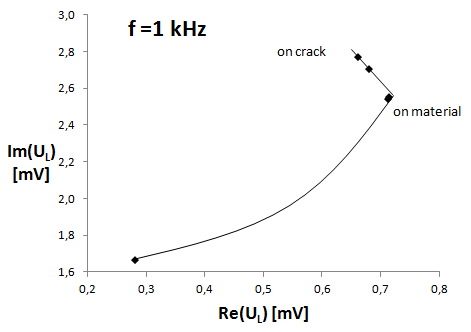
\includegraphics[width=0.50\textwidth]{img/crack1kHz}
	\caption{change in the coil voltage $U_L$ as a function of the position of the probe at a frequency $f=1$ kHz}
	\label{fig:crack1kHz}
\end{figure}

\begin{figure}[htbp]
	\centering
		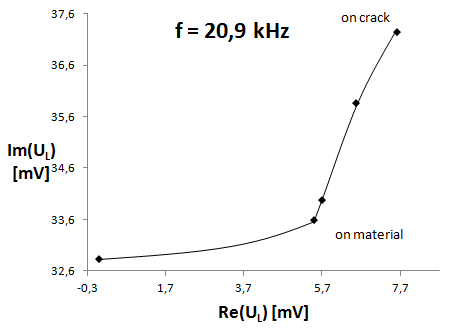
\includegraphics[width=0.50\textwidth]{img/crack21kHz}
	\caption{change in the coil voltage $U_L$ as a function of the position of the probe at a frequency $f=20.9$ kHz}
	\label{fig:crack21kHz}
\end{figure}

\begin{figure}[htbp]
	\centering
		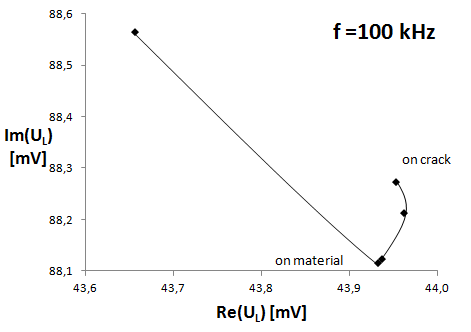
\includegraphics[width=0.50\textwidth]{img/crack100kHz}
	\caption{change in the coil voltage $U_L$ as a function of the position of the probe at a frequency $f=100$ kHz}
	\label{fig:crack100kHz}
\end{figure}

%\begin{figure}[htbp]
	%\centering
		%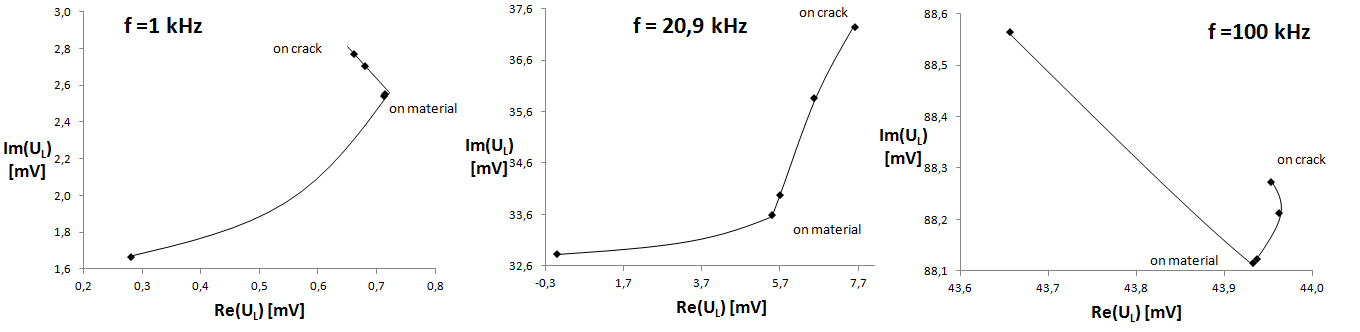
\includegraphics[width=0.90\textwidth]{img/crackAllKHz}
	%\caption{change in the coil voltage $U_L$ as a function of the position of the probe at different frequencies}
	%\label{fig:crackAll}
%\end{figure}



\FloatBarrier
\subsection{Results of resistivity measurement}
In our experiment the change $\Re(\Delta U_L)$ could be measured using the lock-in amplifier.
In order to calculate the constant $C$ in eq. (\ref{eq:resistivity_simp}) we did measurements in three metals with known resistivity: copper, aluminium and tin.
At the measured frequency the skin depth, see eq. (\ref{eq:th_skindepth}), would be around $1\;mm$ for 
$\rho=10^-7$; and the measured conductors were much thicker than this, in the order of one centimetre. So no consideration were taken into the geometry of the conductor.
The measurements along with resistivity and evaluated constant $C$ can be seen below in table \ref{table:measurements}.

\begin{table}[h!]
\caption{Measurements of known metals to evaluate $C$.}
\centering
\begin{tabular}{|c|c|c|c|}
\hline 
\emph{metal} & $\Re(\Delta U_L)$ $(mV)$ & $\rho$ $(\Omega m)$ & $C$ \\ 
\toprule[2pt] 
Copper & 1.56 & 1.68E-8 & 12036 \\ 
\hline 
Aluminium & 1.50  & 2.82E-8 & 8932 \\ 
\hline 
Tin & 0.83  & 1.15E-7 & 2448 \\ 
\hline 
\end{tabular}
\label{table:measurements}
\end{table}
The reader can see that the measured value for the constant $C$ differs by almost a factor of six between
copper and tin; also it is higher for metals with lower resistivity among the metals measured.

The average of these values for $C$ minimizes the summed square error and gives that $C=7805$
This value for $C$ and a measured change in voltage $\Re(\Delta U_L) = 1.22 mV$ for an unknown composition of brass gives $\rho = 2.4432E-8$ compared to brass with 58\% and 63\% copper which have resistivity $5.9E-8 \; \Omega m$ and 
$7.1E-8 \; \Omega m$ respectively.
